\documentclass[preprint,12pt]{elsarticle}
\usepackage{graphicx}
\graphicspath{ {images/} }

\usepackage{geometry}
\geometry{left=0.7cm, right=0.7cm, top=1.7cm, bottom=1.7cm}

\begin{document}
  \begin{figure}[htb]
	\centering
	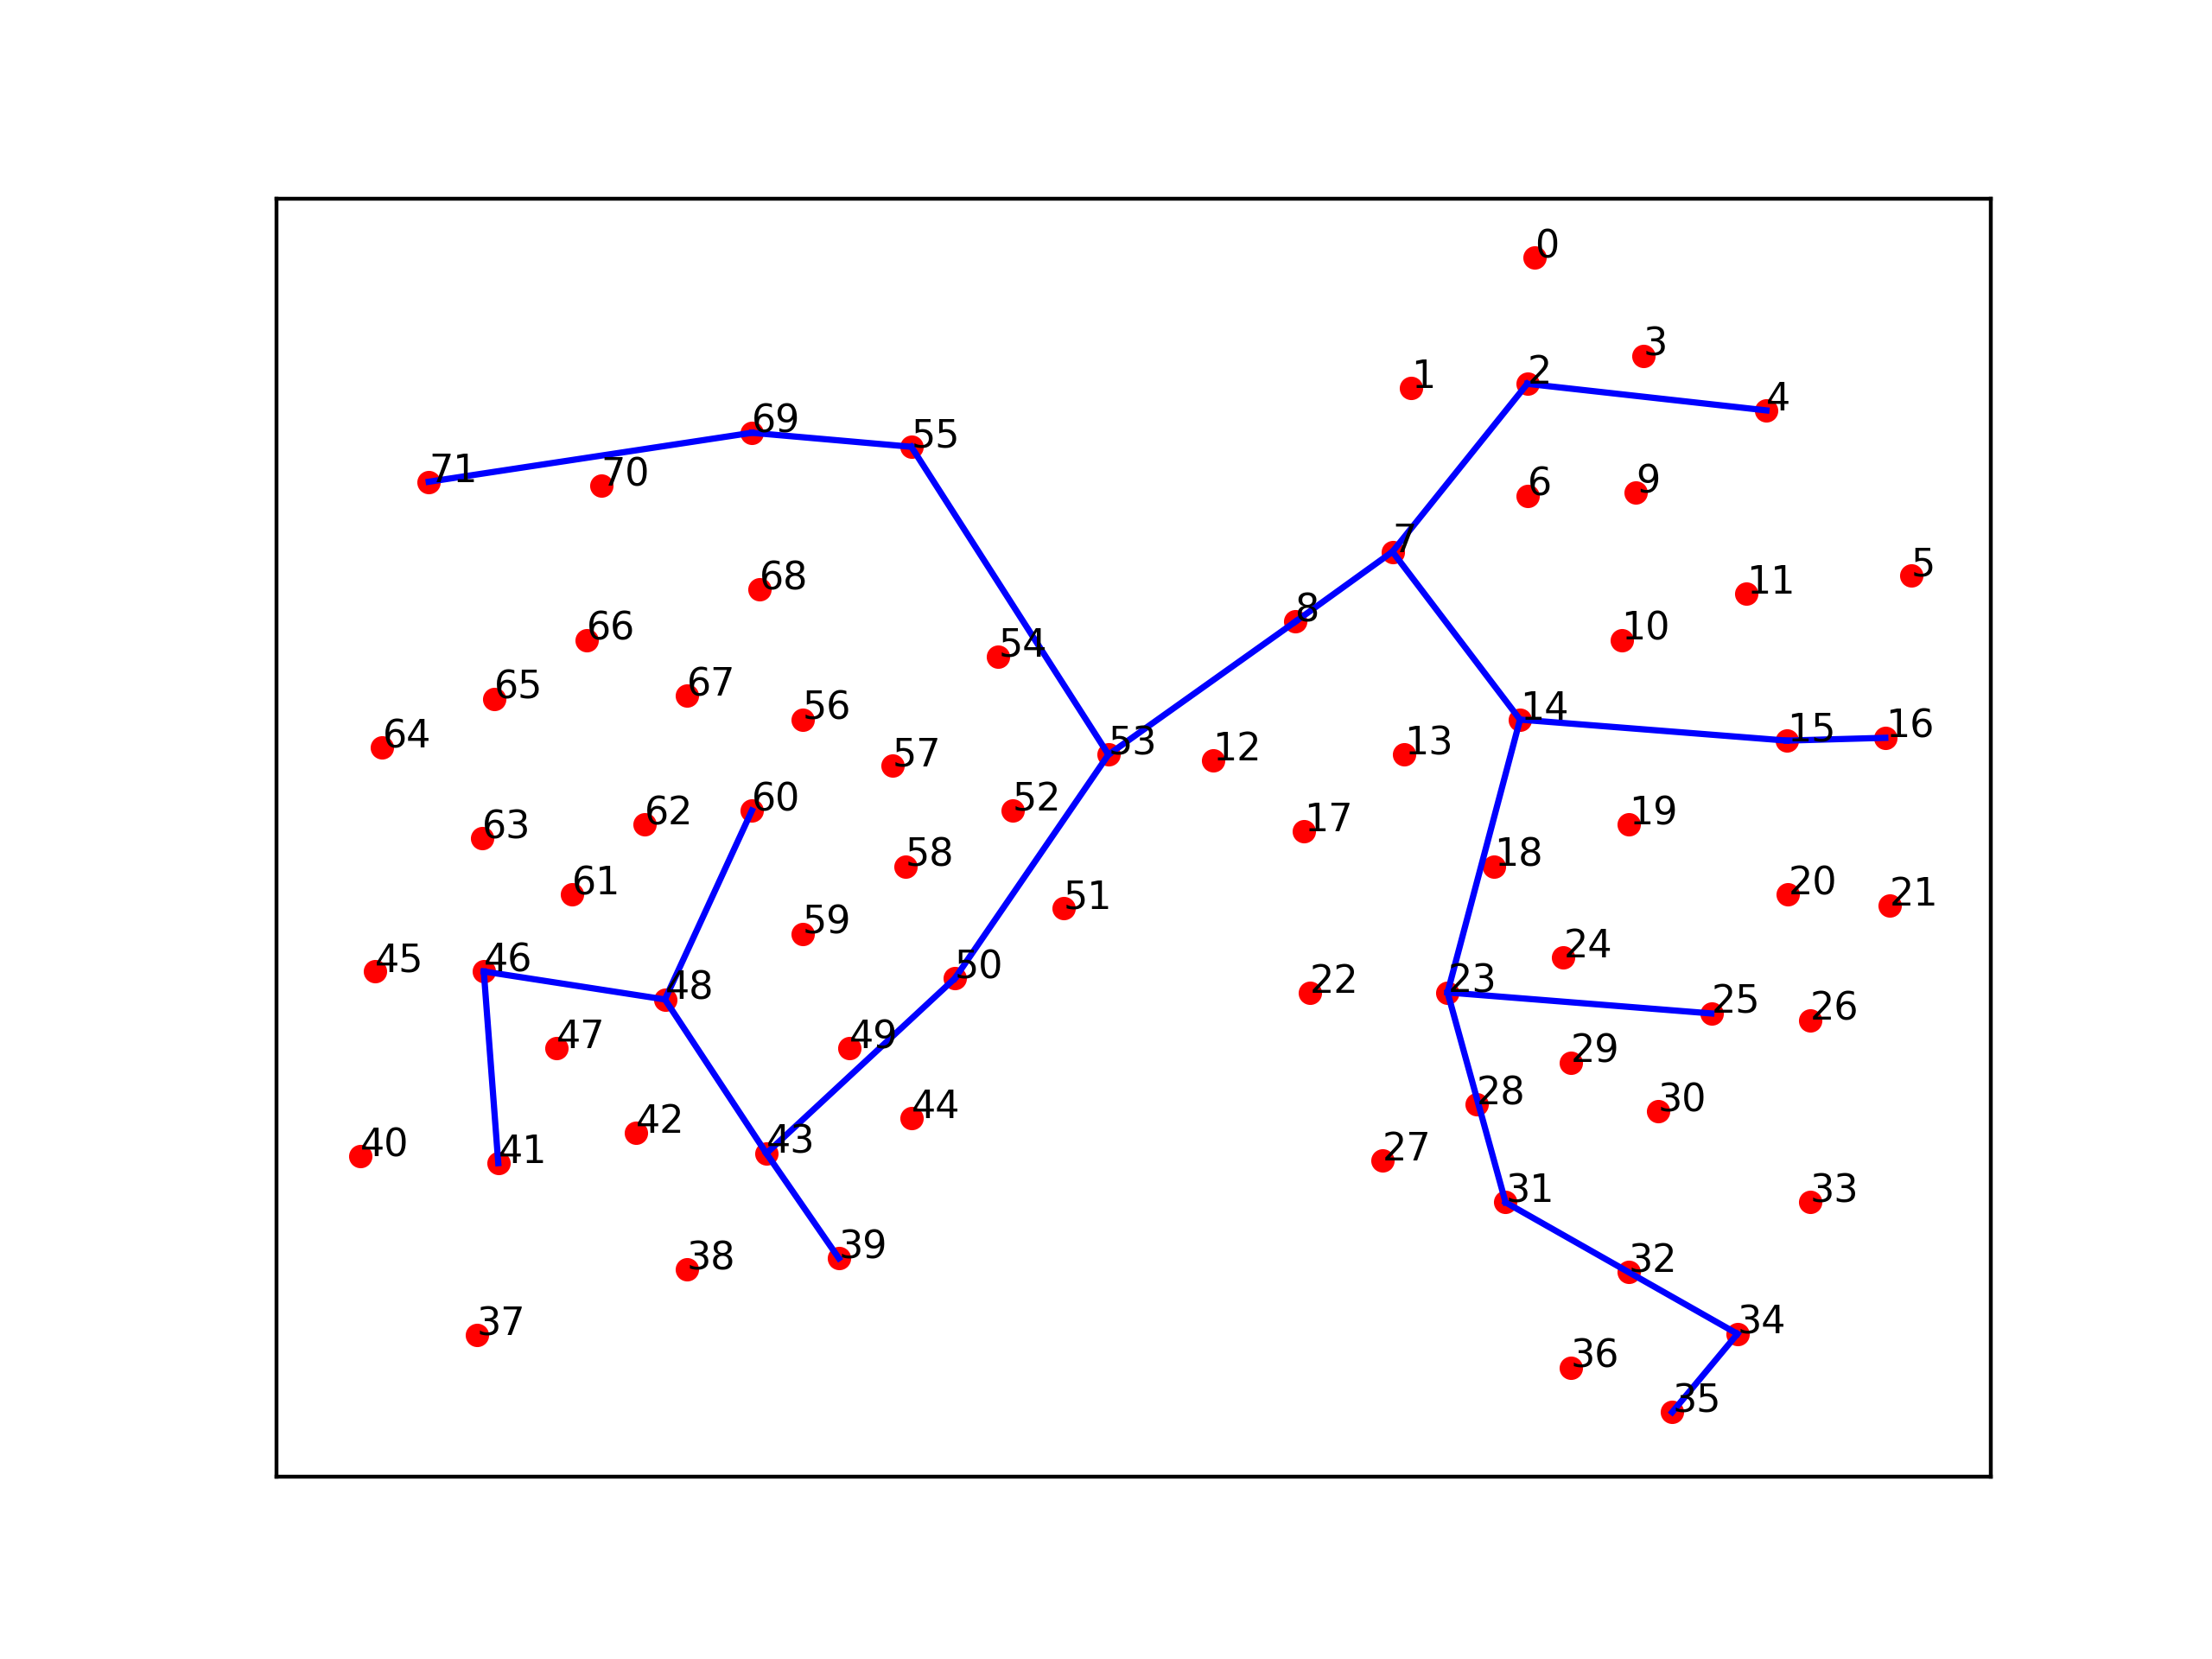
\includegraphics[width=0.45\linewidth]{step1.png}\hspace{-5.6ex}
	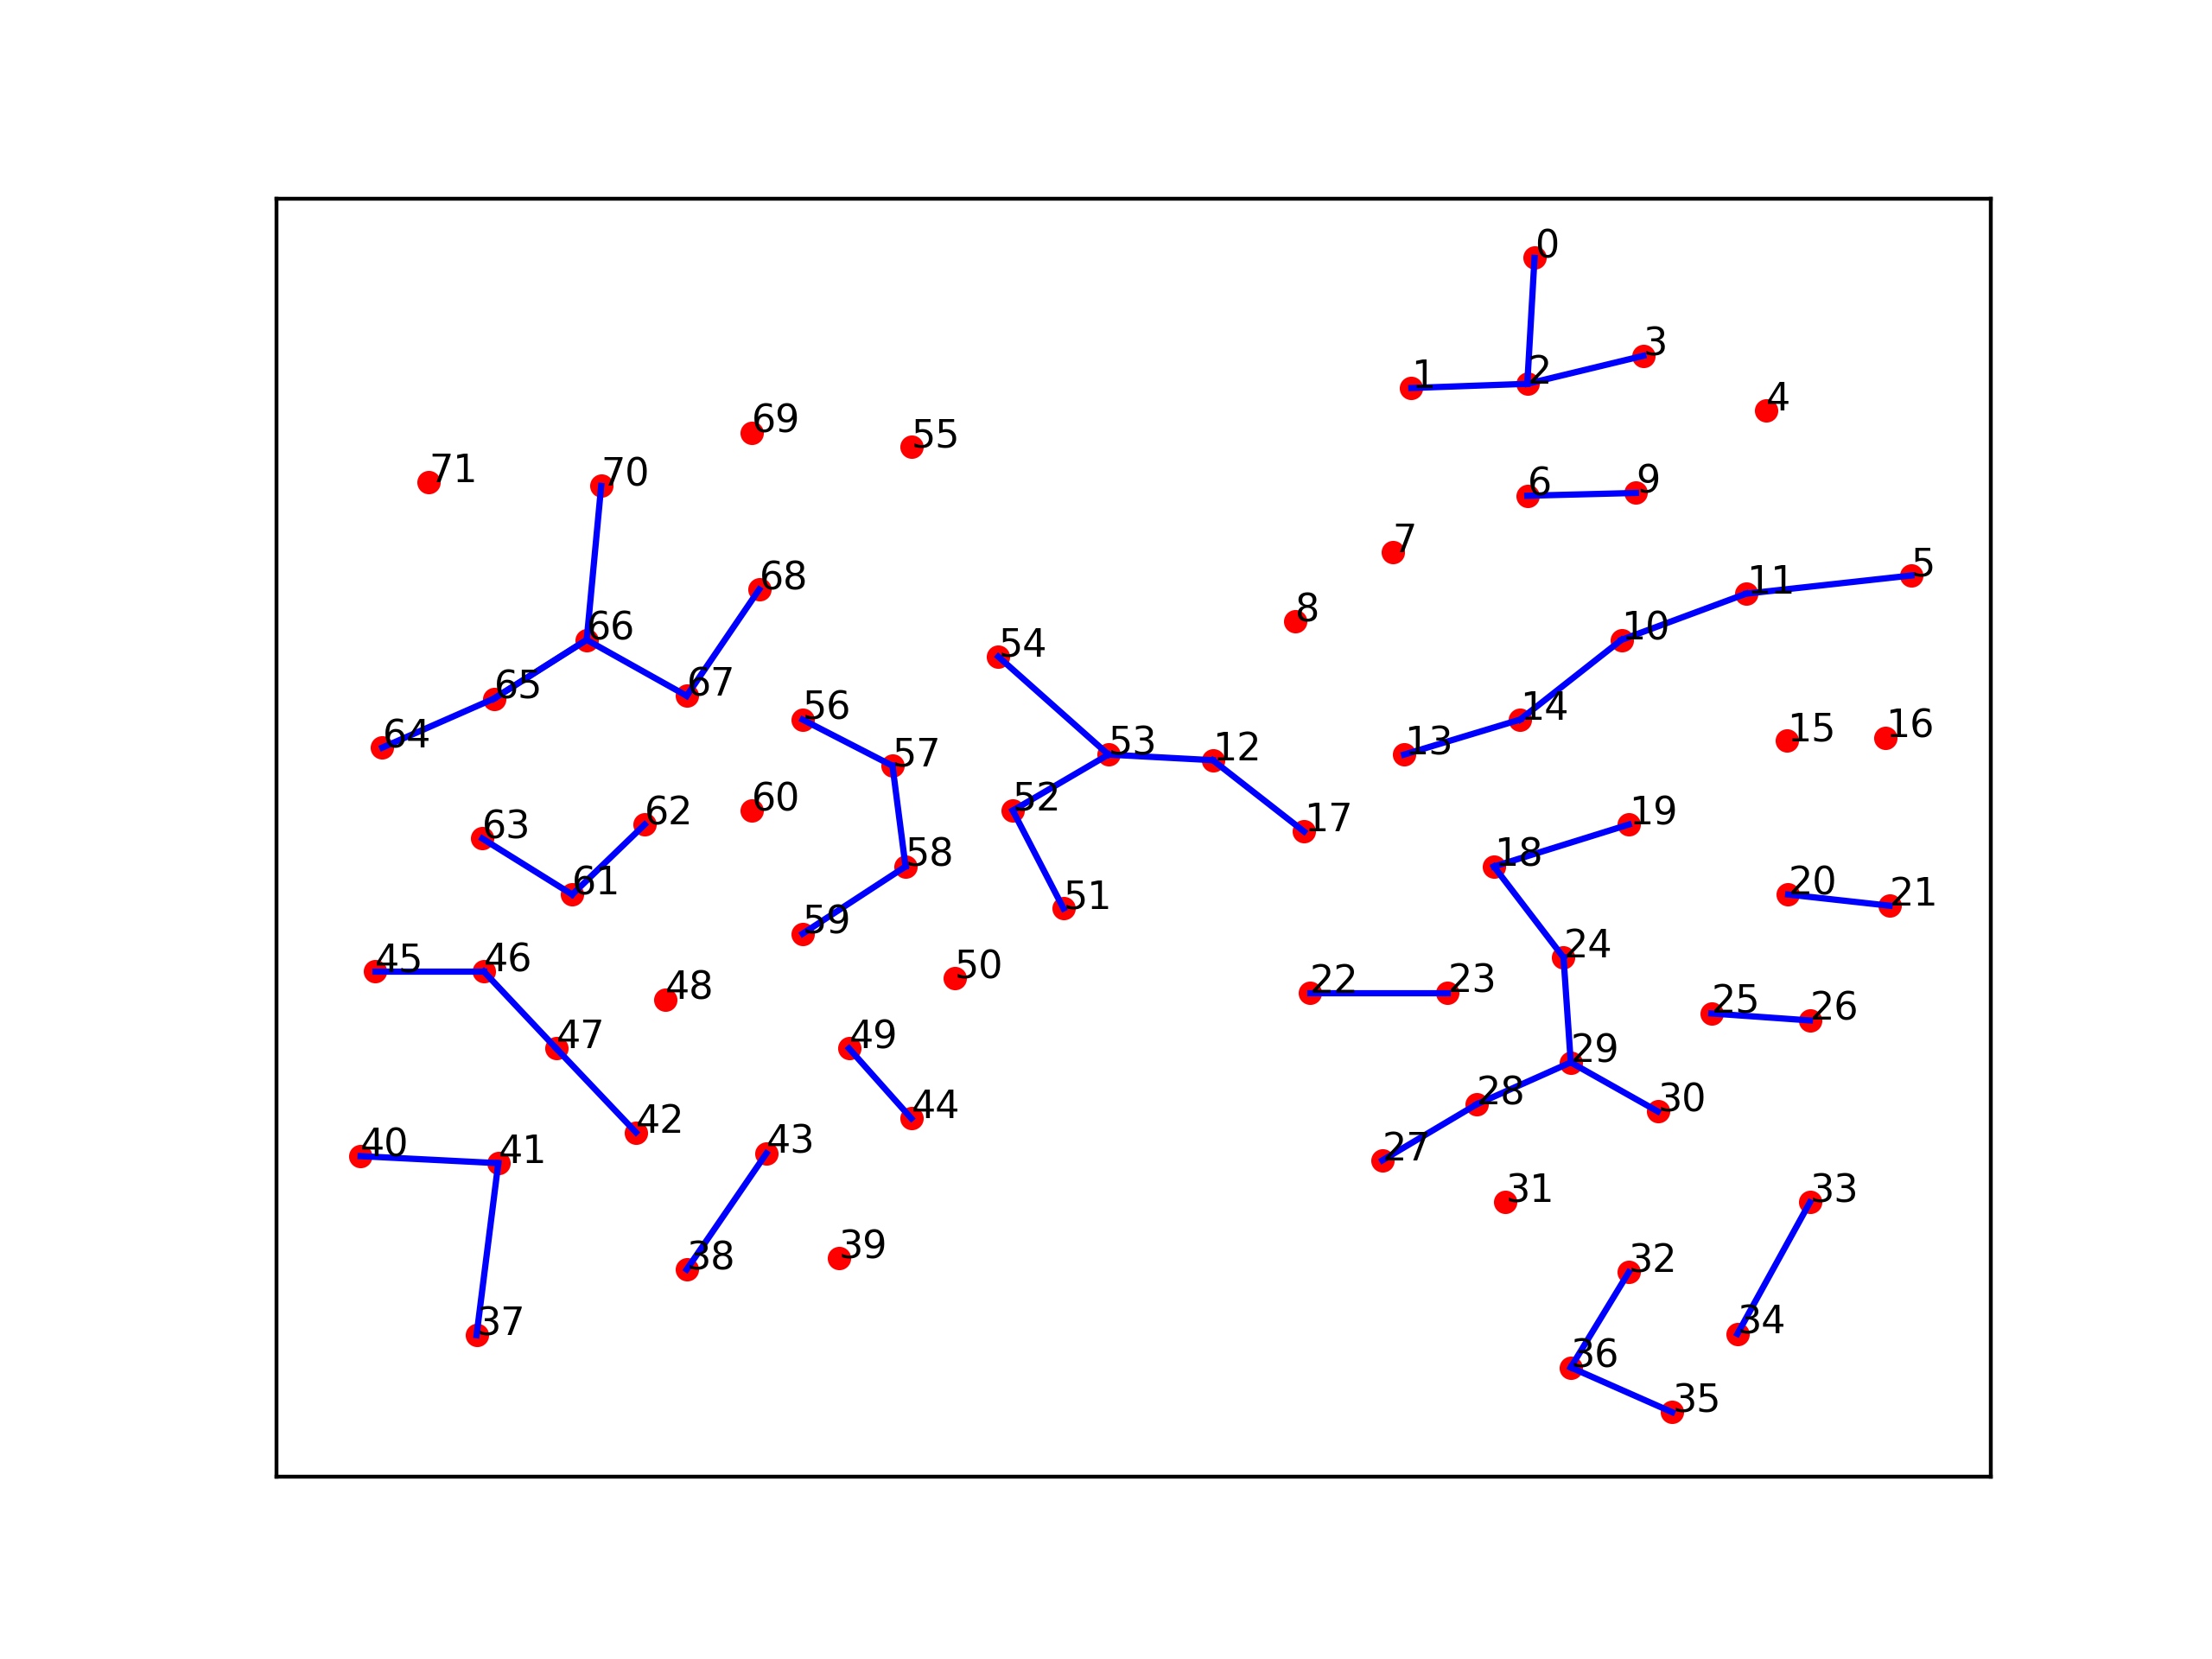
\includegraphics[width=0.45\linewidth]{step2.png}
	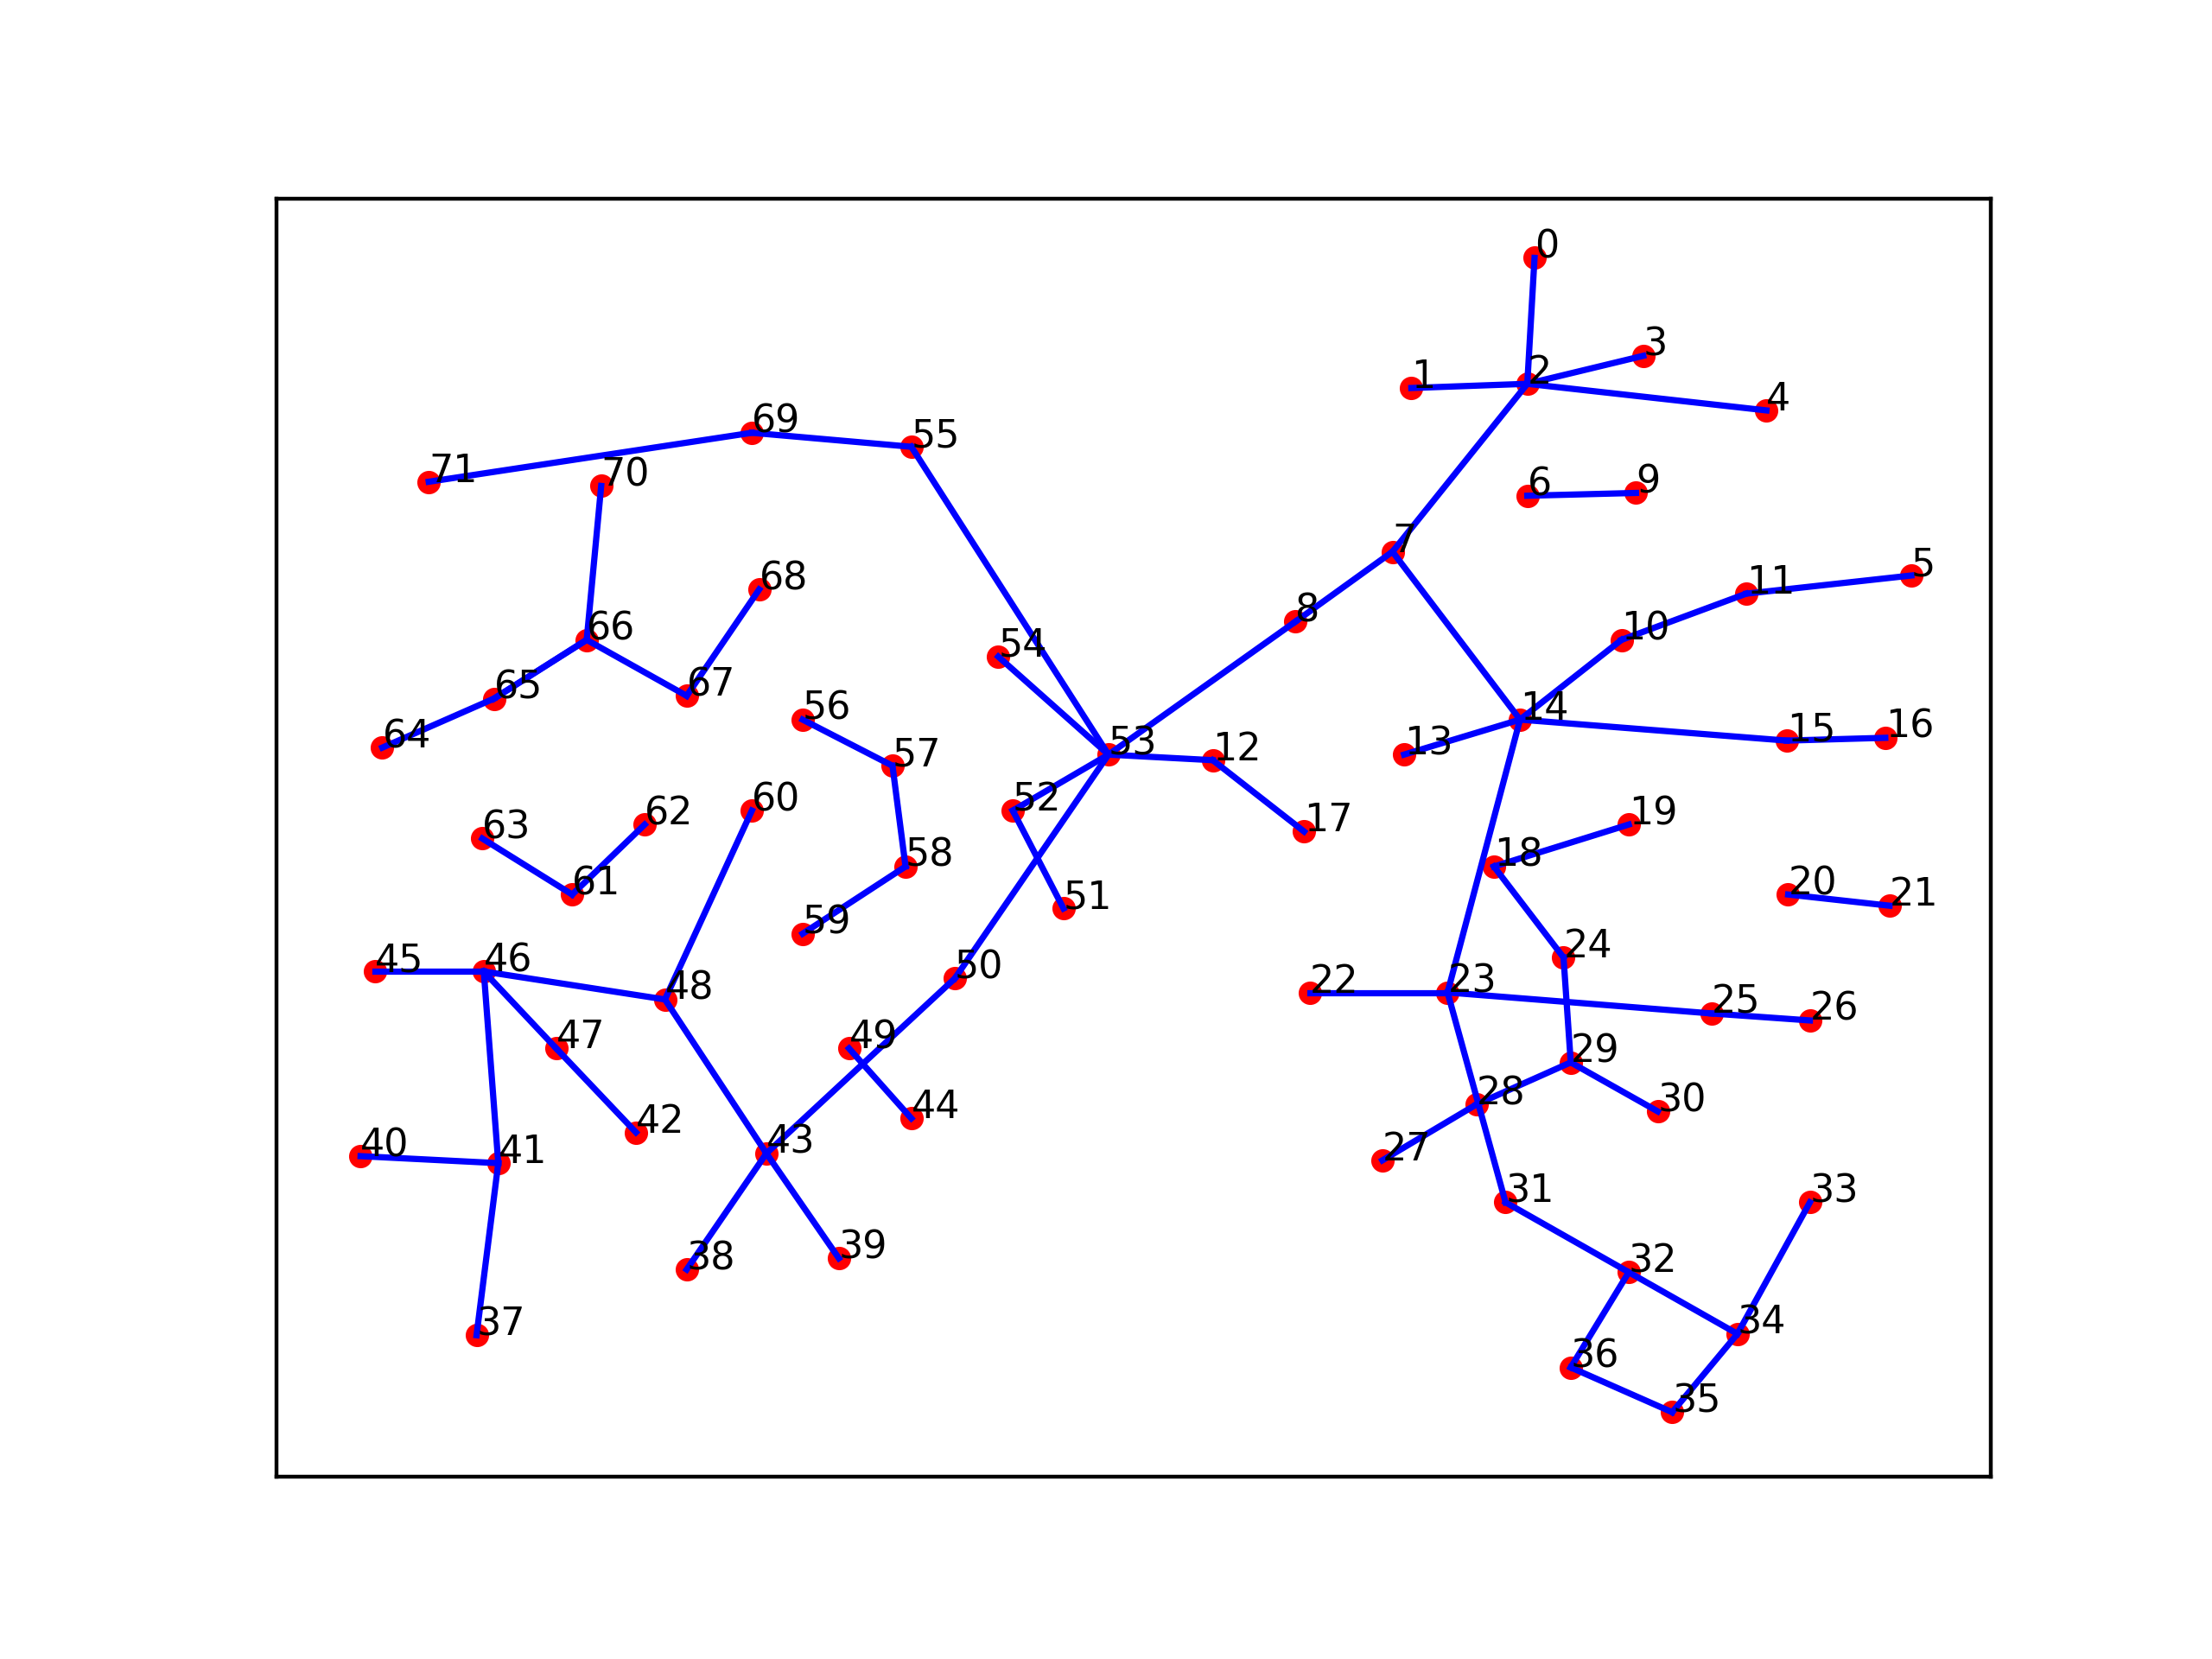
\includegraphics[width=0.45\linewidth]{step3.png}\hspace{-5.6ex}
	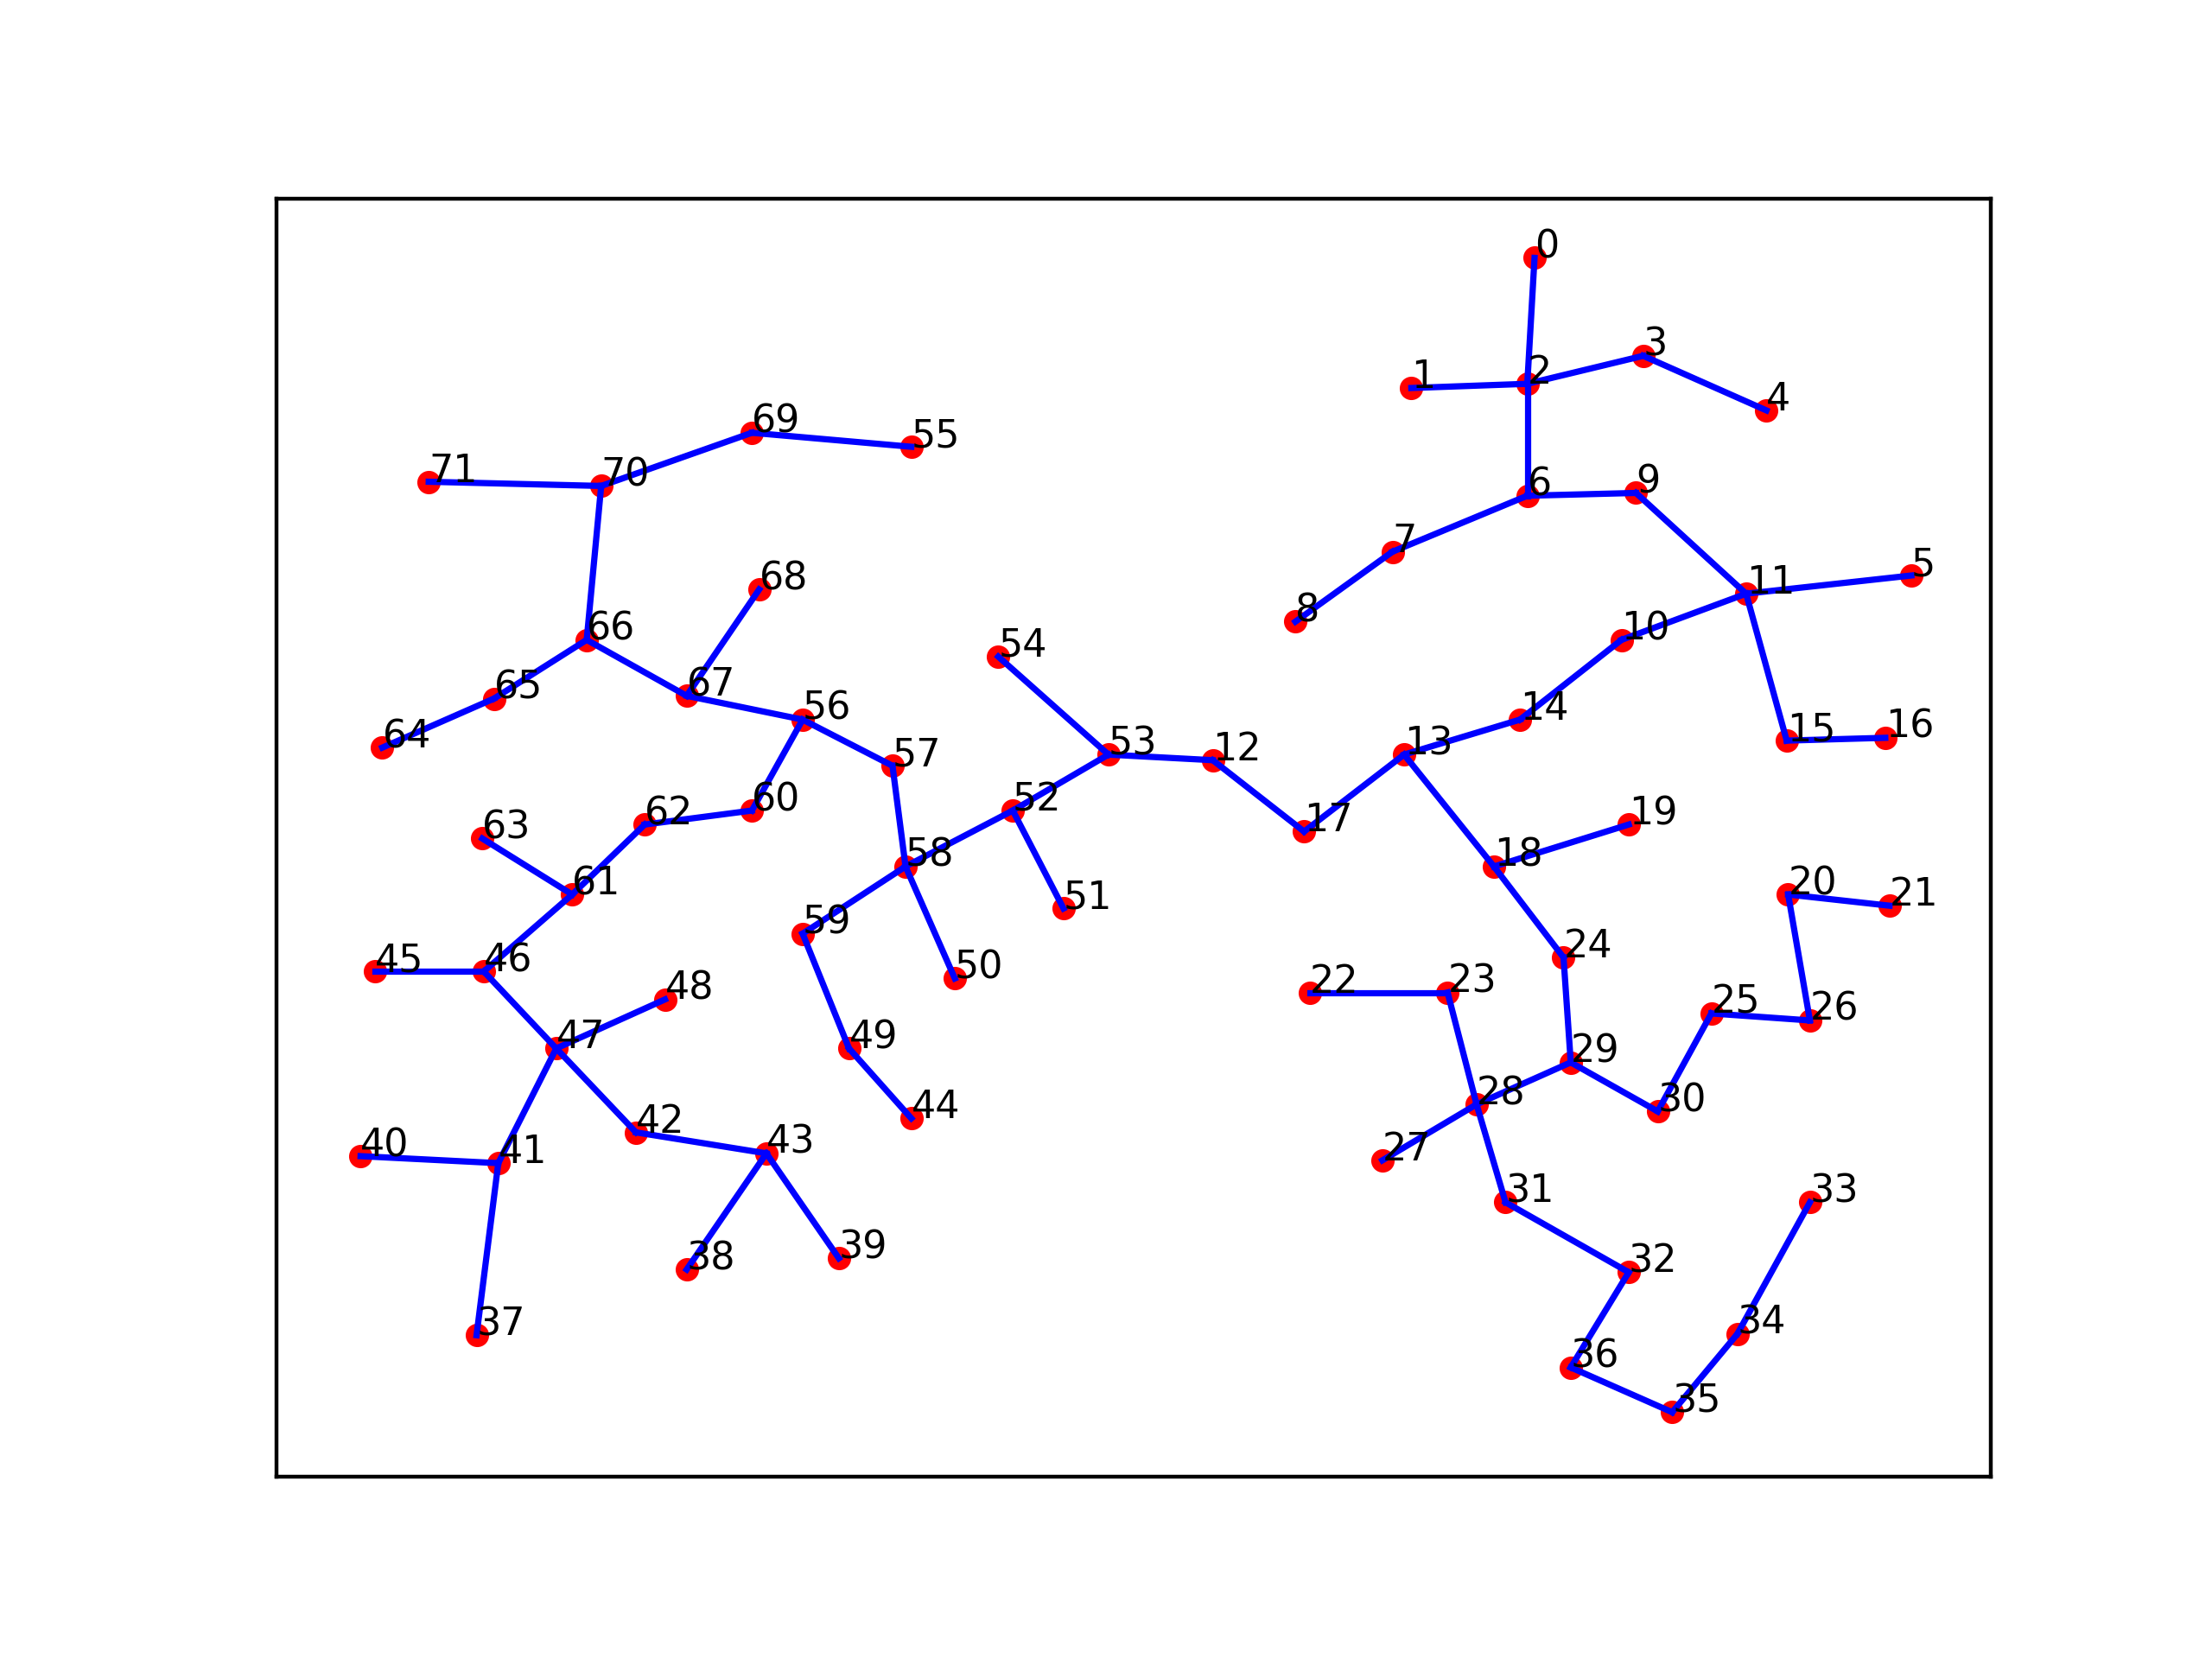
\includegraphics[width=0.45\linewidth]{step4.png}
	% \caption{}
  \end{figure}
 	\begin{figure}[!t]
	 	\subfigure[]{
		\begin{minipage}[b]{0.6\linewidth}
		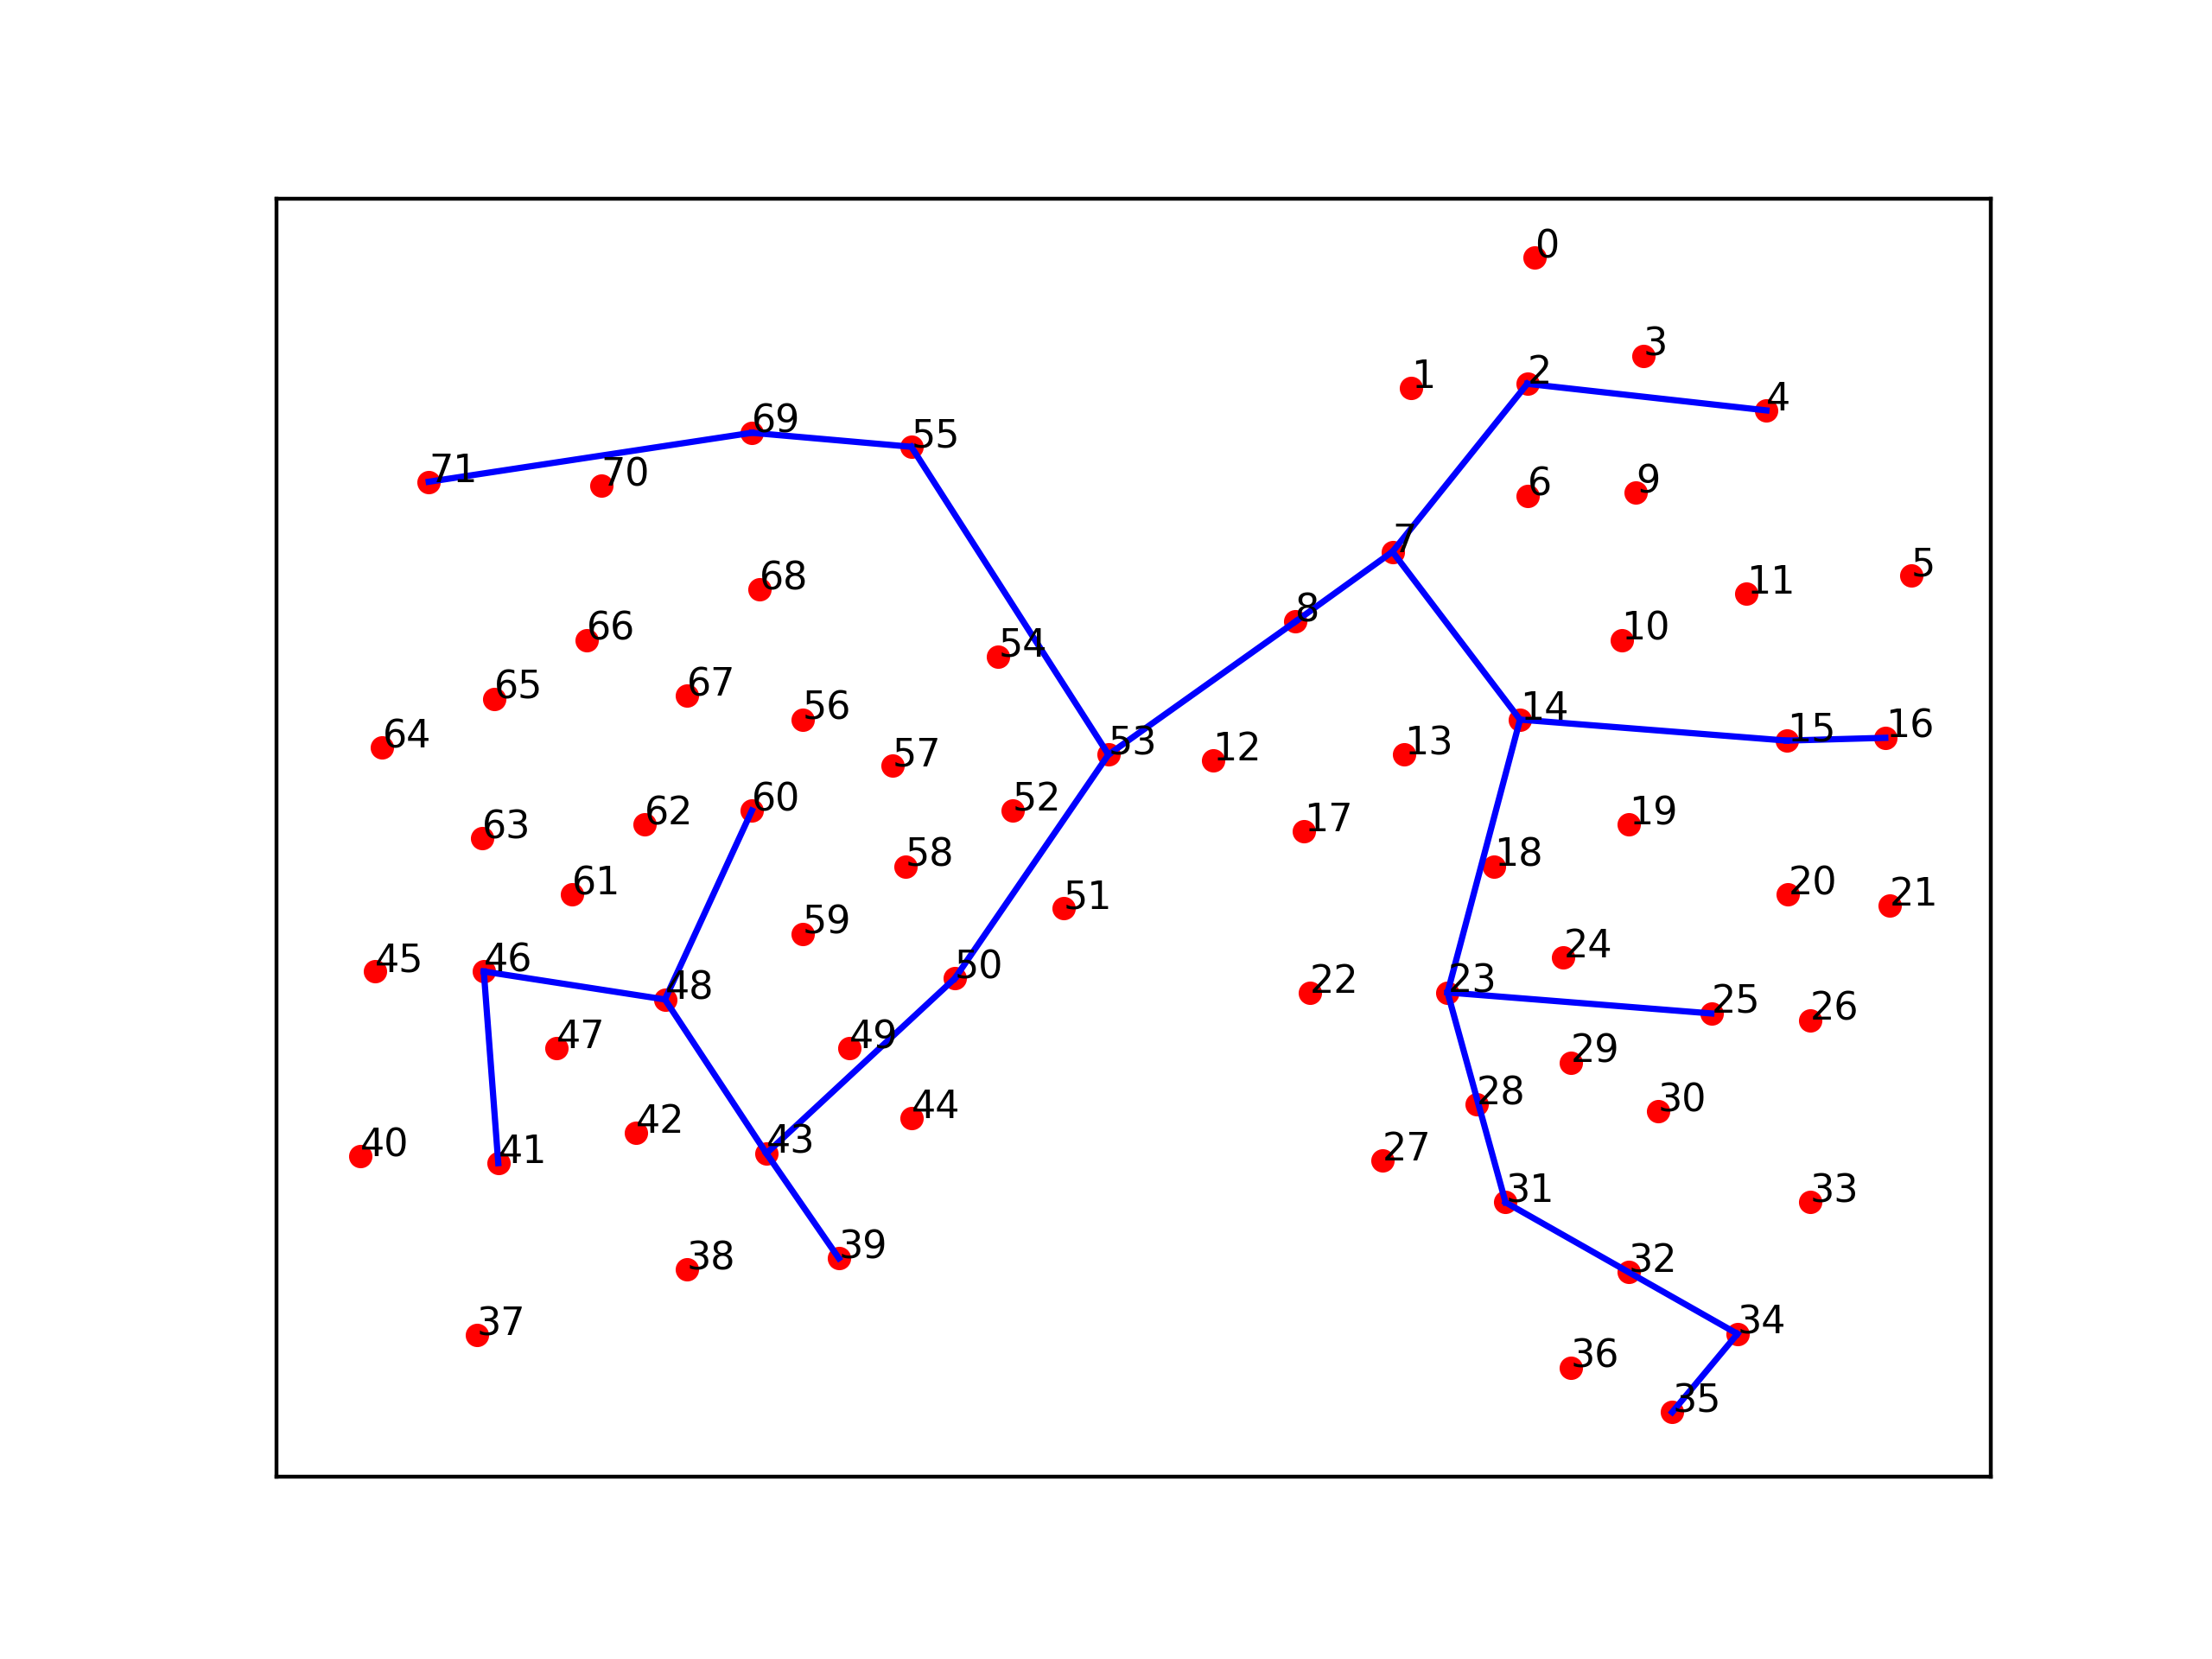
\includegraphics[width=1\linewidth]{step1.png}\vspace{-8pt}
		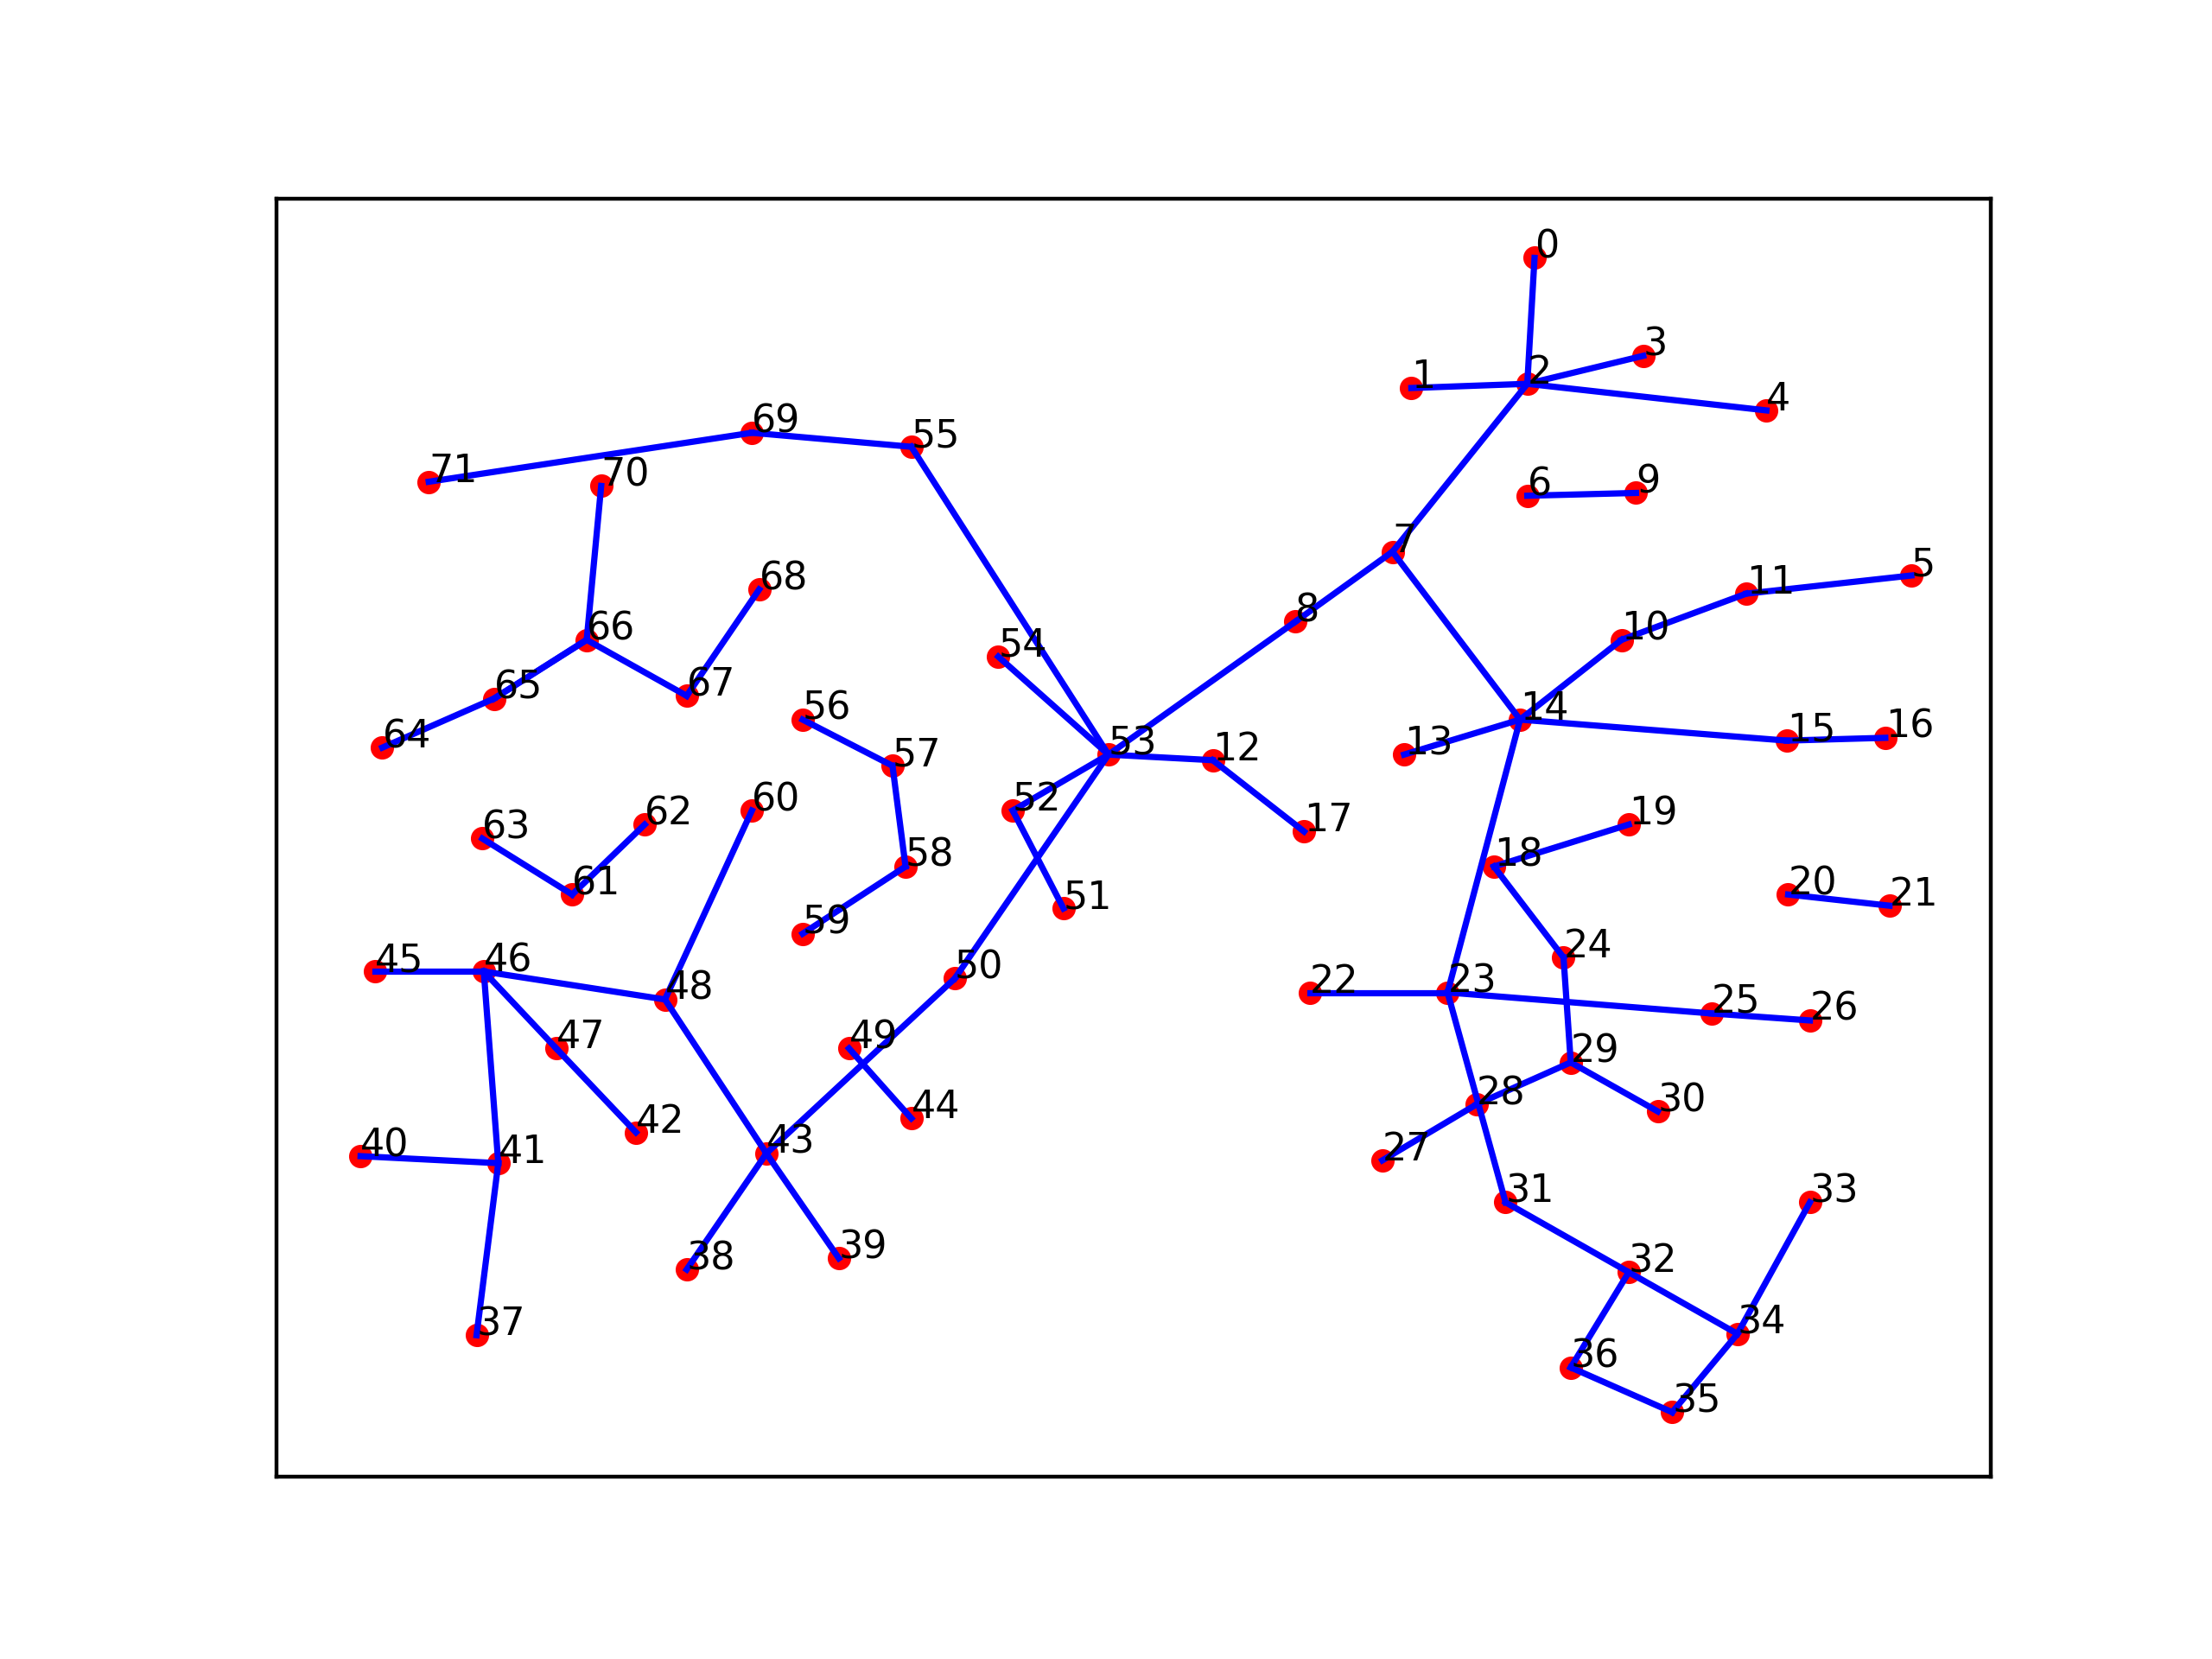
\includegraphics[width=1\linewidth]{step3.png}
		\end{minipage}}
		\subfigure[]{
		\begin{minipage}[b]{0.6\linewidth}
		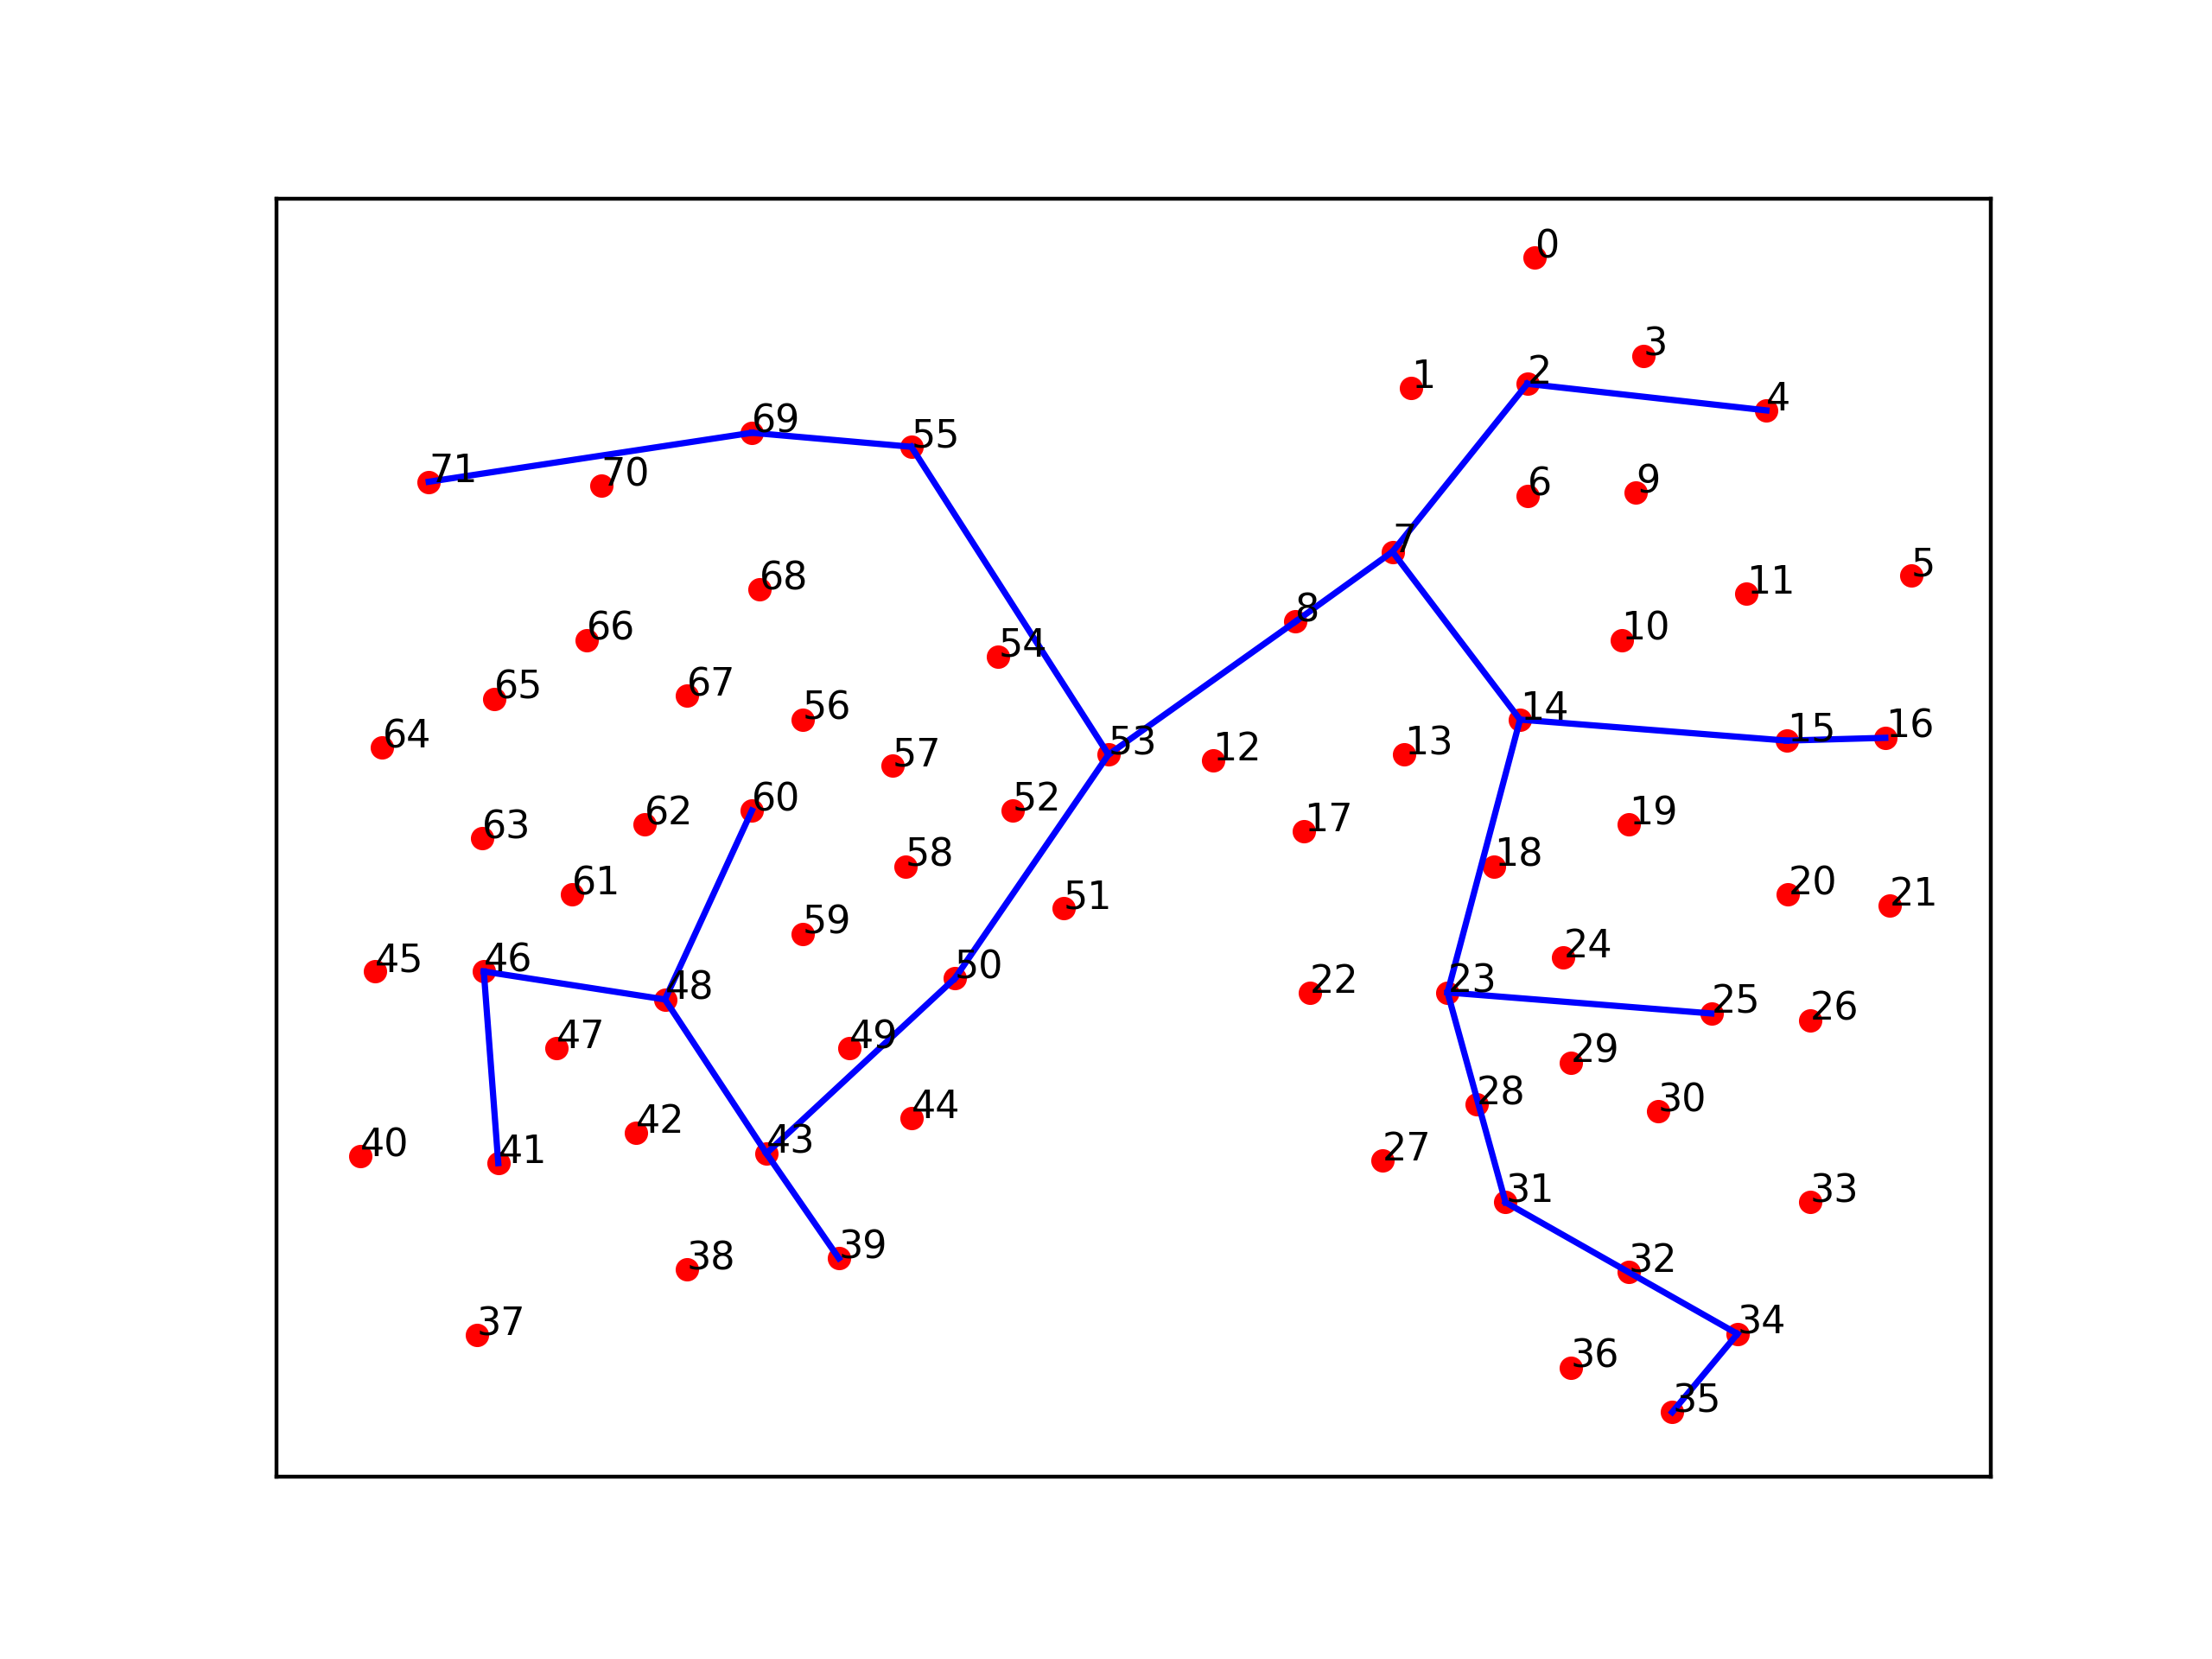
\includegraphics[width=1\linewidth]{step1.png}\vspace{-8pt}
		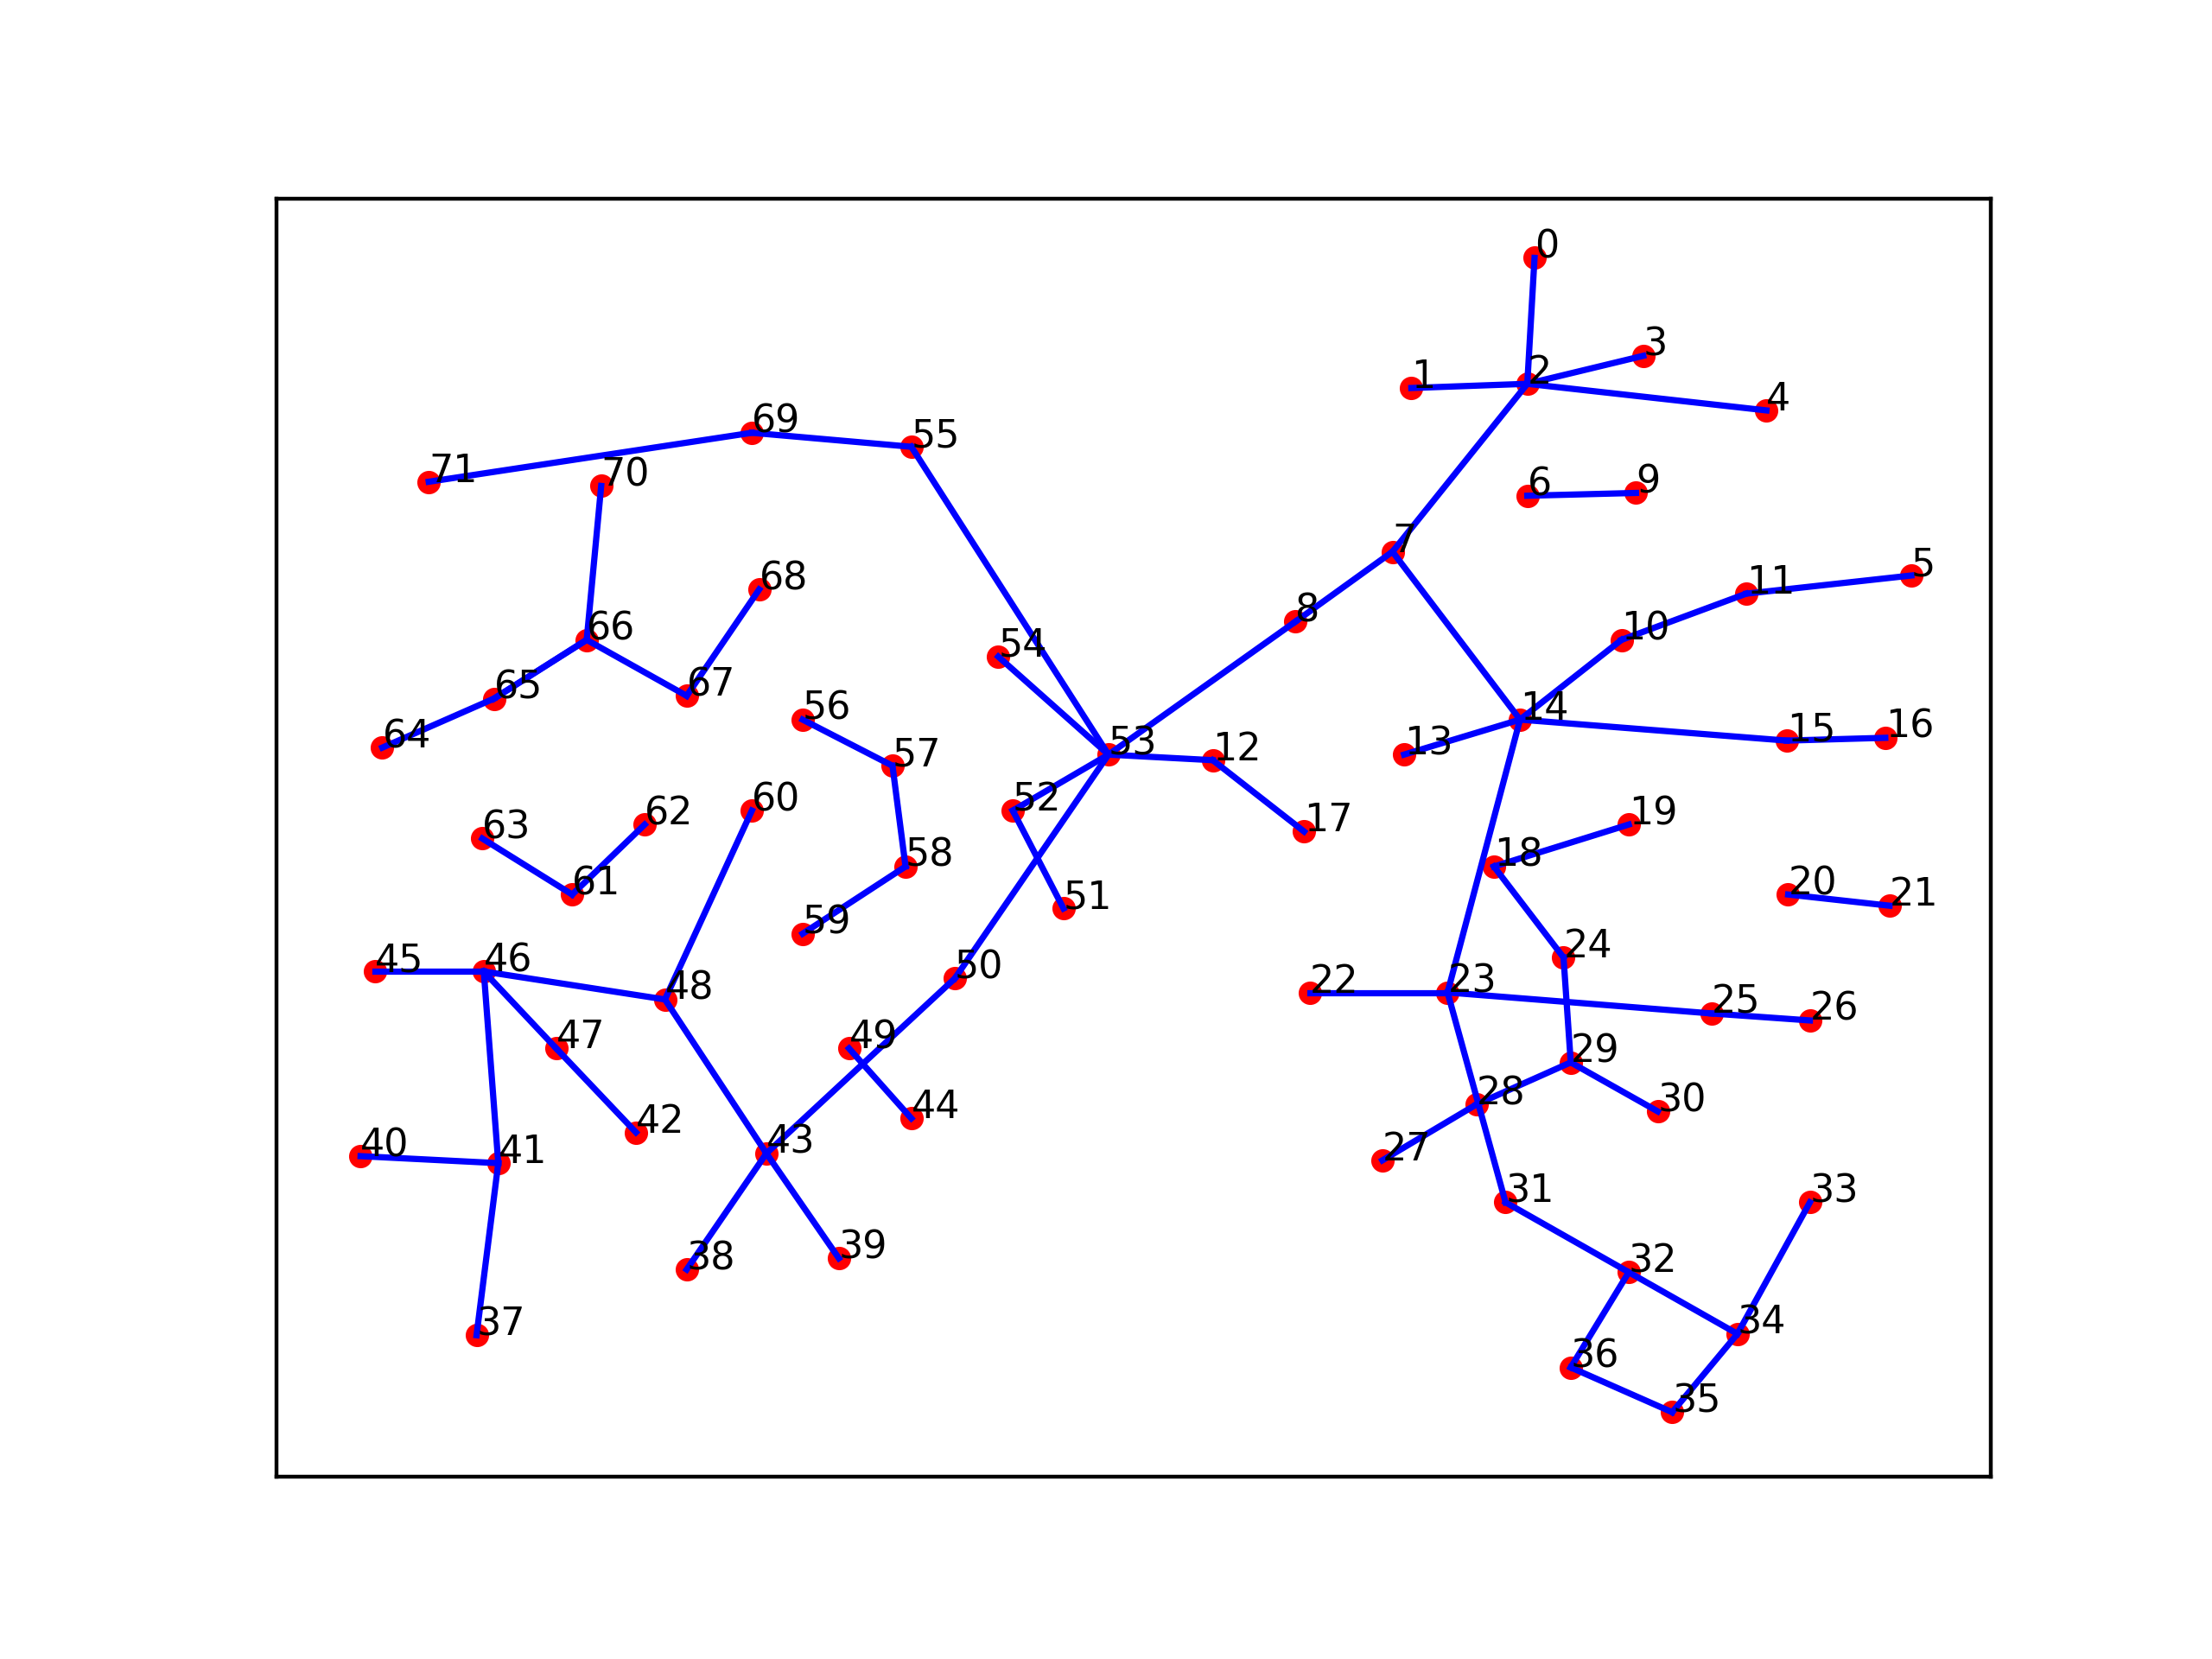
\includegraphics[width=1\linewidth]{step3.png}
		\end{minipage}}
	    \end{figure}
\begin{table}[htb]
	      \centering
	      \caption{clustering result of FMST in different data sets}
	      \label{my-label}
	      \begin{tabular}{|lllll|}
	        \hline
	         Data Name & Rand Index  & Jaccard Index  & Adjust Rand Index & F\-measure  \\ \hline
	         arcene         &  & &  &  \\ 
	         appendicitis   &  & &  &  \\ 
	         banknote       &  & &  &  \\ 
	         breast cancer  &  & &  & \\ 
	         bupa           &  & &  &  \\ 
	         fertility      &  & &  & \\ 
	         haberman       &  & &  &  \\ 
	         hayes-roth     &  & &  & \\ 
	         ionosphere     &  & &  &  \\ 
	         iris           &  & &  & \\ 
	         newthyroid     &  & &  &  \\ 
	         pima           &  & &  & \\ 
	         soybean-small  &  & &  & \\ 
	         wdbc           &  & &  & \\ 
	         wine           &  & &  &  \\ 
	         \hline
	      \end{tabular}
	    \end{table} 
\end{document}
